% Compelling argument demonstrating success criteria met, or well-justified explanation of different direction taken.

% Excellent critical thought and interpretation which substantiate any claims of success.

\label{sec:4}

\section{Review of Success Criteria}
\label{sec:review-of-success-criteria}
My project has met all success criteria as outlined below. Their success is substantiated by the subsequent sections in this chapter.\noparskip
{
    \begin{enumerate}[font=\bfseries]
        \item[1a.]\textbf{Multiple agents will be able to localize themselves within a world using purely visual data.} \\
        My dissertation presents a novel decentralized SLAM system capable of operating using only monocular camera data. This removes the need for large and expensive stereo cameras, LiDAR, or RGBD sensors.
        \label{success-criteria:1a}

        \item[1b.]\textbf{Agents will be capable of communicating with each other to build a shared understanding of the world.} \\
        Agents are capable of efficiently computing map merges and exchanging keyframes to build a shared map of the world. This map can subsequently be used to provide the relative position of peers, as is shown in the real-world collision avoidance experiments.
        \label{success-criteria:1b}

        \item[1c.]\textbf{Agents will be able to act independently, failing gracefully if they lose communication with their peers.} \\
        Agent autonomy is implicitly built into my distributed framework. When communication is degraded, agents will store up map data and send it when communication resumes. This goal is extended by allowing agents to fail gracefully if localization is lost.
        \label{success-criteria:1c}

        \item[2.]\textbf{Evaluate the capabilities of the system compared to a comparable single-agent system.} \\
        This is performed in the \nameref{sec:benchmarking} section. I go beyond the original success criteria by also comparing my system to comparable multi-agent systems, demonstrating my system's superior performance.
        \label{success-criteria:2}

    \end{enumerate}
}
After discussions with my supervisor, \textbf{we decided to not pursue my original project extensions}\footnote[1]{My original extensions can be found in \autoref{sec:project-proposal}}, as we believed that they had either implicitly been achieved during the development of my core deliverables or were no longer relevant to my project.

% Extension 1 and 2 were to ``enable agents to intelligently share information with their peers'' and to ``distribute calculations among the different agents'', which were both already achieved by the \texttt{external keyframe inserter} and \texttt{external map merger} modules. Extension 3 was to develop and test map compression algorithms, however, preliminary testing revealed that data transfer rates were already acceptable. Lastly, we believed that the fourth extension, which involved adding additional sensors as inputs to the system, went against the original 

More importantly, however, \textbf{we were convinced that deploying my system on to physical robots would have far more potential}, and in retrospect, I believe that we made the correct choice. Operating my system in real-time on a distributed platform proves its applicability in real-world scenarios, and shows that my system can adapt to the noisy and unpredictable conditions of the real world, greatly improving its credibility. Moreover, deploying my system on to the Cambridge RoboMasters provides evidence of how my software engineering choices have enabled my system to be reproducible on a variety of hardware, instead of just my laptop.

\section{Benchmarking}
\label{sec:benchmarking}
This section will benchmark the performance of my system when run on industry-standard visual SLAM datasets. All evaluations are run using only monocular camera data. The Central Management Interface is used to stream the dataset to the agents and my library \textit{Multi-Agent EVO} is used to provide the Absolute Trajectory Error (ATE) metric, as defined by \autocite{6385773}.

\subsection{EuRoC Machine Hall}
\label{sec:euroc-machine-hall}
The EuRoC Machine Hall dataset \autocite{burri2016euroc} is one of the most widely used visual SLAM datasets, providing a 752x480 20fps video feed and millimeter-level ground truth data at 20hz. The camera rig is attached to a Micro Aerial Vehicle which flies through a machine room of approximately 15x15 meters in size. In line with other research, I simulate a multi-agent dataset by running the Machine Hall 01-03 scenarios in parallel on three agents.

\autoref{fig:euroc-mh-01-03-5-trials} presents the root mean square (RMS) absolute trajectory error and total data transfer of my distributed system running this dataset. \textbf{The median RMS ATE is 5.9cm over the 279-meter total trajectory length}, demonstrating my system's very impressive accuracy. The 5 trials' ATE have a 1.4cm spread around the median respectively, demonstrating the repeatability and robustness of my system.

\begin{figure}[h]
    \centering
    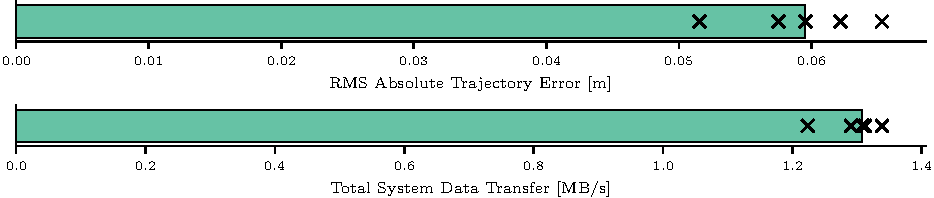
\includegraphics[width=0.8\linewidth]{figures/comparison_apr11_mh_trajectory_b.pdf}

    \caption{Plot the RMS absolute trajectory error and total data transfer rate of running the EuRoC Machine Hall 01-03 dataset 5 times on my system.}
    \label{fig:euroc-mh-01-03-5-trials}
\end{figure}

\begin{figure}[h]
    \centering
    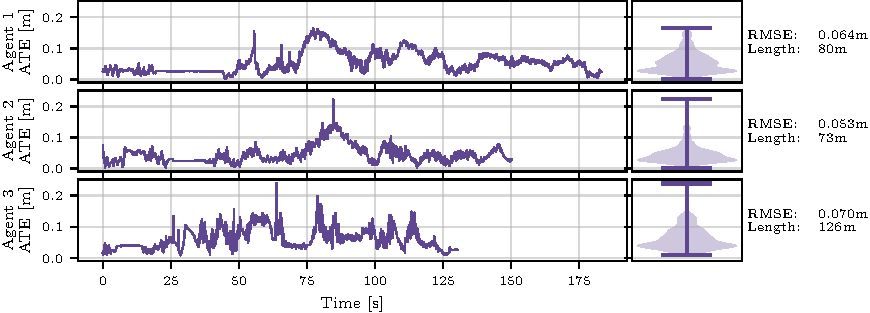
\includegraphics[width=0.85\linewidth]{figures/apr11_mh_trajectory_b_line_plot.pdf}

    \caption{Plot of my system's absolute trajectory error (ATE) with respect to the ground truth when running the EuRoC Machine Hall 01-03 scenarios in parallel on three agents.}
    \label{fig:euroc-mh-01-03-line-plot}
\end{figure}

To further analyze the characteristics of my SLAM system, we will focus on an individual trial. \autoref{fig:euroc-traj} displays the full trajectory of the three agents compared to the ground truth, demonstrating my system's high global accuracy and relative positioning. \autoref{fig:euroc-mh-01-03-line-plot} plots the ATE as the trial progresses. \textbf{It is clear that my system is performing SLAM as opposed to simple visual odometry} as the ATE returns to the baseline at the end of the trial when the agents return to their starting positions, with no accumulated drift.


We now analyze the network usage presented in \autoref{fig:euroc-mh-01-02-bandwith}. Initially, the agents send bag of word information before quickly detecting a merge opportunity. The agents exchange their maps, which can be seen in the large initial spike in network bandwidth. After a successful merge, they begin exchanging keyframes. The rate of keyframe data fluctuates depending on how much new area the agents are exploring.


Along with sending keyframes, the agents sporadically send map points to refine their map alignment. This occurs less frequently the longer system runs due to the additive increase multiplicative decrease method used to schedule map alignments, described in the \nameref{sec:map-alignment-refiner} section. However, the size of the messages also grows over time due to the growing map.


\begin{figure}[h]
    \centering
    \captionsetup{format=plain}
    \begin{subfigure}[t]{0.5\linewidth}
        \centering
        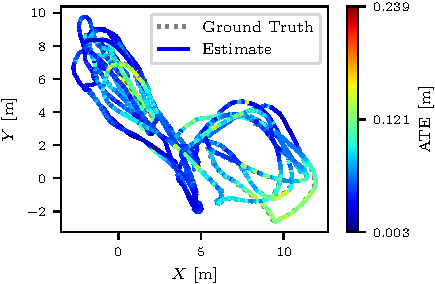
\includegraphics[width=0.9\linewidth]{figures/apr11_mh_trajectory_b_trajectory.pdf}
        \caption{Estimated trajectory and ground truth.}
    \end{subfigure}\hfill%
    ~
    \begin{subfigure}[t]{0.45\linewidth}
        \centering
        \raisebox{0.15in}{%
            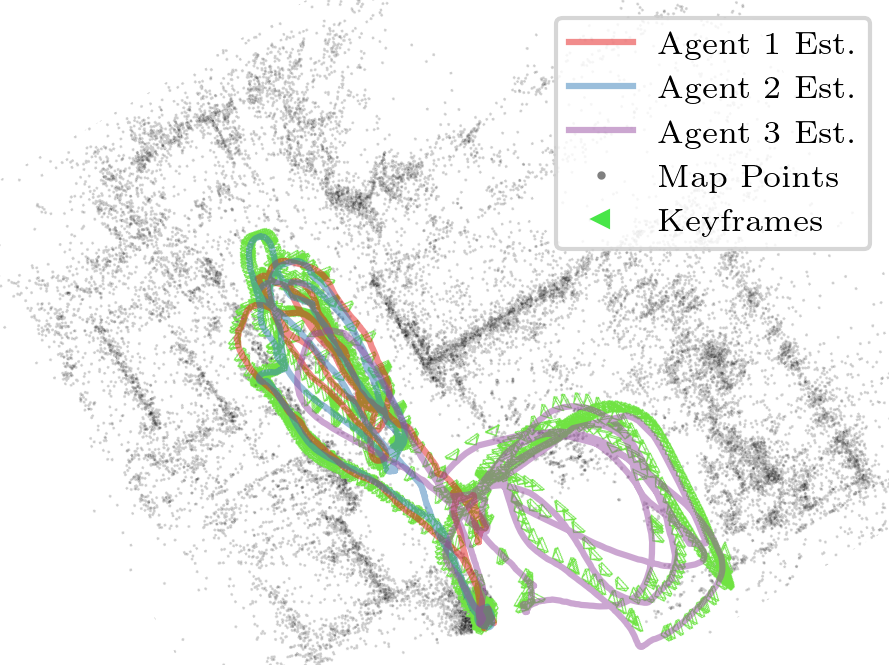
\includegraphics[width=0.9\linewidth]{figures/apr11_mh_trajectory_b_trajectory_overlay.png}
        }
        \caption{Final map and individual agent trajectories.}
    \end{subfigure}

    \caption{EuRoC Machine Hall 01-03. A video recording of the trial gives a 3D visualization of the map and is available at 1m06s of the supplementary video\protect\footnotemark[1].}
    \label{fig:euroc-traj}

\end{figure}
\begin{figure}[h]
    \centering
    \begin{subfigure}[b]{0.55\linewidth}
        \centering
        \marginbox{0 0 0 0} {
            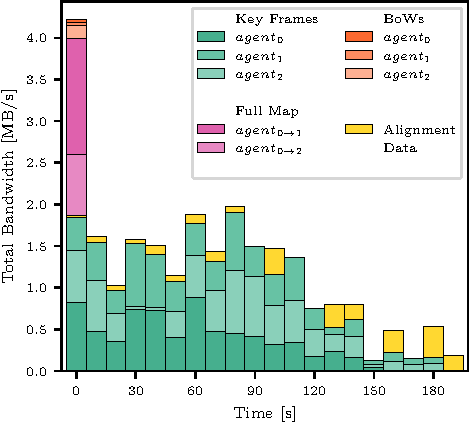
\includegraphics[width=0.9\linewidth, valign=t]{figures/apr11_mh_trajectory_b_bandwith.pdf}
        }
        \caption{Total system data over time, segregated by message type}
    \end{subfigure}%
    ~
    \begin{subfigure}[b]{0.45\linewidth}
        \centering
        \adjustbox{valign=t, width=0.9\linewidth}{
            \marginbox{0.2in 0 0 0} {

                \def\arraystretch{1.2}
                \begin{tabular}{ |c|l|r|r| }
                    \cline{3-4}
                    \multicolumn{2}{}{}                       & \multicolumn{1}{|c|}{KB} & \multicolumn{1}{|c|}{Avg. KB/s}         \\
                    \hline
                    \multirow{3}{*}{Key Frames}               & $agent_0$                & 69,971                          & 351.9 \\
                                                              & $agent_1$                & 63,908                          & 321.4 \\
                                                              & $agent_2$                & 65,164                          & 327.7 \\
                    \hline
                    \multirow{3}{*}{BoWs}                     & $agent_0$                & 371                             & 1.9   \\
                                                              & $agent_1$                & 437                             & 2.2   \\
                                                              & $agent_2$                & 1,496                           & 7.5   \\
                    \hline
                    \multirow{2}{*}{Full Map}
                                                              & $agent_{0\to1}$          & 13,953                          & 70.2  \\
                                                              & $agent_{0\to2}$          & 7,319                           & 36.8  \\
                    \hline
                    \multicolumn{2}{|c|}{Alignment Data}      & 22,560                   & 113.6                                   \\
                    \hline
                    \multicolumn{2}{|c|}{\textbf{Total Data}} & \textbf{245,218}         & \textbf{1,233.1}                        \\
                    \hline
                \end{tabular}
            }
        }
        \caption{Total system data by message type}
        \vfill

        \adjustbox{valign=b, width=0.9\linewidth}{
            \marginbox{0.2in 0 0 0.3in} {
                \def\arraystretch{1.2}
                \begin{tabular}{ |l|r|r|r|r| }
                    \cline{2-5}
                    \multicolumn{1}{}{} & \multicolumn{2}{|c|}{Sent} & \multicolumn{2}{|c|}{Received}                                                               \\
                    \cline{2-5}
                    \multicolumn{1}{}{} & \multicolumn{1}{|c|}{KB}   & \multicolumn{1}{|c|}{Avg. KB/s} & \multicolumn{1}{|c|}{KB} & \multicolumn{1}{|c|}{Avg. KB/s} \\
                    \hline
                    $agent_0$           & \textbf{114,585}           & \textbf{576.2}                  & \textbf{131,005}         & \textbf{658.8}                  \\
                    \hline
                    $agent_1$           & \textbf{64,345}            & \textbf{323.6}                  & \textbf{173,554}         & \textbf{872.8}                  \\
                    \hline
                    $agent_2$           & \textbf{66,660}            & \textbf{335.2}                  & \textbf{164,606}         & \textbf{827.7}                  \\
                    \hline
                \end{tabular}
            }
        }
        \caption{Data by agent}
    \end{subfigure}%

    \caption{Bandwidth used by the EuRoC Machine Hall 01-03 scenarios running on my SLAM system.}
    \label{fig:euroc-mh-01-02-bandwith}
\end{figure}

% just randomly put here lol
\footnotetext[1]{Supplementary video URL: \url{https://cam-diss.s3.amazonaws.com/video.mp4}}

\subsection{TUM-VI Rooms}
\label{sec:tum-rooms}
The TUM visual-inertial dataset \autocite{8593419} consists of handheld fisheye 512x512 video with ground truth data. As before, I only use monocular visual data and combine the Room 1-3 sessions to simulate a multi-agent dataset. The ``room'' environment is used for this evaluation, which is a 3x3 meter motion capture lab with plain flat walls and some posters hung up. There is less texture in this environment than the machine hall, making visual-only SLAM difficult. As seen in the full trajectory estimate given in \autoref{fig:tum-traj}, parts of the room are revisited dozens of times by different agents, allowing us to evaluate our system's ability to relocalize agents within previously mapped environments.

\autoref{fig:tum-room-01-03-5-trials} shows that the RMS ATE is very tightly clustered around the median of 6.95cm, with one outlier caused by an agent in that trial having a slightly un-optimal map merge. The tight clustering is most likely due to the small environment with areas being revisited many times, allowing the shared map to converge on a very similar solution each time. The lower data transfer rate of 0.84 MB/s is also due to the small environment, resulting in the agents having to share less information.

\begin{figure}[h]
    \centering
    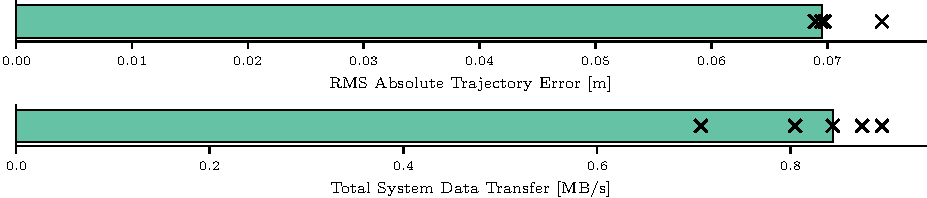
\includegraphics[width=0.8\linewidth]{figures/comparison_apr11_tum_room_trajectory_a.pdf}

    \caption{Plot the RMS ATE and Total Data Transfer rate of running the TUM-VI Rooms 1-3 dataset 5 times on my system.}
    \label{fig:tum-room-01-03-5-trials}
\end{figure}

\begin{figure}[h]
    \centering
    \captionsetup{format=plain}
    \begin{subfigure}[t]{0.5\linewidth}
        \centering
        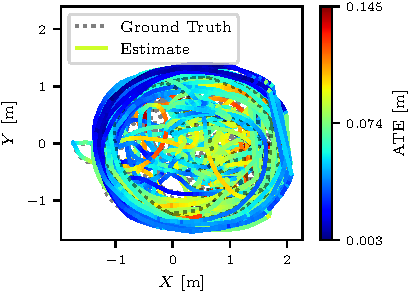
\includegraphics[width=0.9\linewidth]{figures/apr11_tum_room_trajectory_a_trajectory.pdf}
        \caption{Estimated trajectory and ground truth.}
    \end{subfigure}\hfill%
    ~
    \begin{subfigure}[t]{0.45\linewidth}
        \centering
        \raisebox{0.15in}{%
            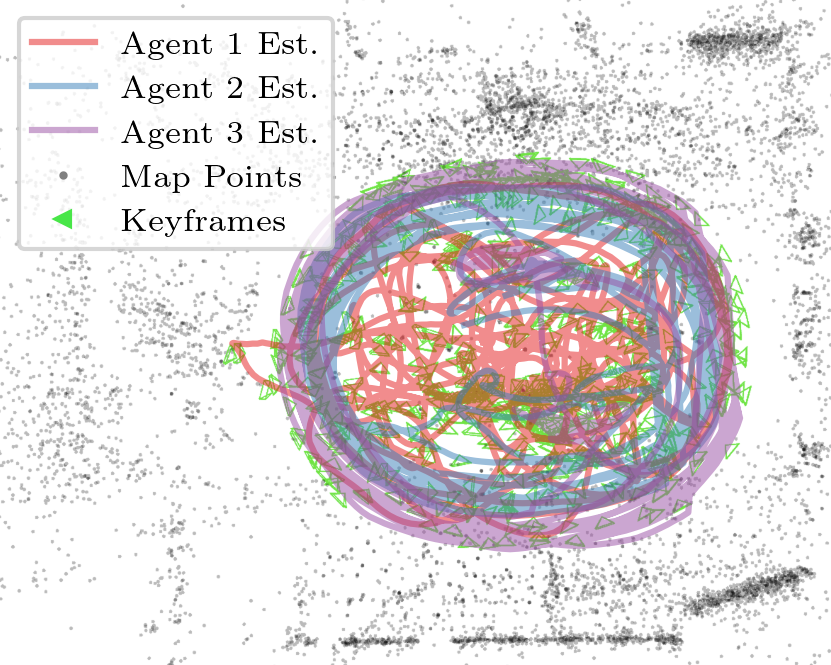
\includegraphics[width=0.9\linewidth]{figures/apr11_tum_room_trajectory_a_trajectory_overlay.png}
        }
        \caption{Final map and individual agent trajectories.}
    \end{subfigure}

    \caption{TUM-VI Rooms 01-03. A video recording of the trial gives a 3D visualization of the map and is available at 0m04s of the supplementary video\protect\footnotemark[1].}
    \label{fig:tum-traj}
\end{figure}
\footnotetext[1]{Supplementary video URL: \url{https://cam-diss.s3.amazonaws.com/video.mp4}}

Once again, we focus on an individual trial to further evaluate my system. \autoref{fig:tum-room-01-03-line-plot} shows that there is \textbf{no long-term error built up}, demonstrating that my system is successfully localizing agents within the shared map and performing long-term map point association.

\begin{figure}[h]
    \centering
    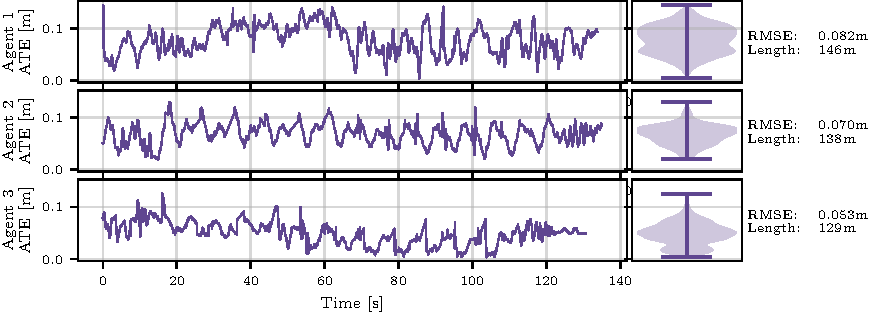
\includegraphics[width=0.85\linewidth]{figures/apr11_tum_room_trajectory_a_line_plot.pdf}

    \caption{Plot of my system's absolute trajectory error (ATE) with respect to the ground truth when running the TUM-VI Room 1-3 scenarios in parallel on three agents.}
    \label{fig:tum-room-01-03-line-plot}
\end{figure}

The data transfer characteristics are given by \autoref{fig:tum-rooms-01-03-bandwith} in the appendix, and yield similar conclusions to that of the EuRoC Machine Hall dataset. The only difference to note is the smaller key frame and alignment data transfer rate due to the smaller environment.

\section{Comparison to Related Work}
\label{sec:comparison-to-related-work}

As discussed in the \nameref{sec:relevant-work} section, to the best of my knowledge, my system is the only publically available decentralized monocular vision SLAM system. This makes direct comparisons with other multi-agent SLAM systems difficult, as they rely on more accurate but bulky sensors such as stereo cameras and LiDAR. However, this section still attempts to compare my system to the latest research in the field to give context on its performance relative to other state-of-the-art systems.

\subsection{CCM-SLAM}
\label{sec:ccm-slam}
Centralized Collaborative Monocular SLAM (CCM-SLAM) (2019) from the ETH Zurich Vision for Robotics Lab \autocite{schmuck2019ccm} is the most comparable multi-agent SLAM system in recent literature and is well-cited within the field. To my knowledge, it is the most recent monocular vision-capable multi-agent SLAM system.

It is important to note that CCM-SLAM is a \textit{centralized} system, significantly simplifying their multi-agent SLAM problem compared to my distributed system. \textbf{Nevertheless, my system outperforms CCM-SLAM in terms of RMS absolute trajectory error, as presented in \autoref{fig:comparison-to-multi-agent-systems}.} Notably, CCM-SLAM failed all 5 trials of the TUM-VI Rooms dataset, due to its inability to relocalize an agent if localization is lost. This greatly reduces the robustness of their system as tracking is often lost in real-world use cases due to motion blur or a lack of visible features. The latter is the reason for CCM-SLAM's failures on the TUM-VI dataset, as the environment contains plain walls which may cause a brief loss of tracking.

% In terms of total data transfer, my system is 32\% higher than CCM-SLAM. However, this could easily be reduced as there have been almost no attempt to optimize the data transfer efficiency of my system.

\subsection{VINS-Mono Multisession SLAM}
VINS-Mono (2018) \autocite{8421746} is a popular open-source \textit{single-agent} monocular vision SLAM system with multisession capabilities. This allows multiple datasets to be played consecutively, with each session building upon the map built by the previous sessions. This is an easier problem than multi-agent SLAM, where the sessions are run in parallel and agents share their maps in real-time. In addition, VINS-Mono requires inertial data, so it is not a purely monocular vision system. \textbf{As presented in \autoref{fig:comparison-to-multi-agent-systems}, my system still outperforms VINS-Mono multisession.}


\begin{figure}[h]
    \centering
    \def\arraystretch{1.2}
    \small
    \begin{tabular}{ |c|c|c|c| }
        \cline{2-4}
        \multicolumn{1}{c|}{}    & \textbf{My system} & CCM-SLAM$^1$ & VINS-Mono$^2$ \\
        \hline
        EuRoC Machine Hall 01-03 & \textbf{0.059}     & 0.077        & 0.074         \\
        \hline
        Tum-VI Rooms 1-3         & \textbf{0.070}     & FAILED       & 0.256         \\
        \hline
    \end{tabular}

    \caption{RMS absolute trajectory error of my SLAM system relative to comparable state-of-the-art multi-agent systems. All results are taken as the median of 5 trials.\captionbreak $^1$CCM-SLAM is a centralized system, as opposed to my decentralized system. \\ $^2$VINS-Mono is a single-agent SLAM system run in multisession mode. Additionally, it requires inertial data, unlike the other two systems.}
    \label{fig:comparison-to-multi-agent-systems}
\end{figure}

The difference in performance is particularly pronounced in the TUM-VI Rooms dataset. This was due to their system only merging agents' maps locally – once an agent moved away from the merge site, it began creating an entirely new map instead of reusing the map built by the previous agent. Therefore, the global consistency of the shared map was lacking which resulted in the high RMS ATE of the combined trajectories.

\subsection{Comparison to Single-Agent SLAM Systems}
We would hypothesize that a multi-agent SLAM system will have higher accuracy than a comparable single-agent system, due to the increased available data. However, the reality is far more complex than this simple assumption. \autoref{fig:comparison-to-single-agent-systems} presents my multi-agent system's errors compared to ORB-SLAM3 running the datasets individually. ORB-SLAM3 is widely regarded as the most accurate single-agent SLAM system currently available, so it is no surprise that it performs very well.

It can be observed that my system only has a marginal improvement in error over the single-agent system, which I hypothesize is the result of the varying ability among agents to utilize the shared map. For example, the TUM-VI Room environment is very small and areas of the map are revisited dozens of times in one session. This reduces the benefit of the increased data provided by a multi-agent system as a single session already observes more than enough data to build an accurate map of the world.

We see a significant improvement in error for the EuRoC Machine Hall 02 session, likely due to the 02 agent closely following the 01 agent. Conversely, the 01 session's error is not reduced, likely because it leads the way for the 02 session. The 03 session explores a separate part of the environment from the other sessions, so a similar performance is to be expected.

\begin{figure}[h]
    \captionsetup{format=plain}
    \begin{minipage}[c]{0.5\textwidth}
        \centering

        \adjustbox{valign=t, width=\linewidth}{
            \marginbox{0in 0 0 -0.2in} {
                \def\arraystretch{1.2}
                \small
                \begin{tabular}{ |l|l|l| }
                    \cline{2-3}
                    \multicolumn{1}{c|}{} & \textbf{My system}$^1$ & ORB-SLAM3$^2$  \\
                    \hline
                    EuRoC MH 01           & 0.051                  & \textbf{0.049} \\
                    EuRoC MH 02           & \textbf{0.048}         & 0.099          \\
                    EuRoC MH 03           & \textbf{0.058}         & 0.062          \\
                    \hline
                    TUM-VI Room 1         & 0.072                  & \textbf{0.071} \\
                    TUM-VI Room 2         & \textbf{0.048}         & 0.050          \\
                    TUM-VI Room 3         & \textbf{0.041}         & 0.042          \\
                    \hline
                \end{tabular}
            }
        }
    \end{minipage}\hfill
    \begin{minipage}[c]{0.48\textwidth}
        \caption{Comparison of RMS ATE from my distributed SLAM system and the single-agent ORB-SLAM. All results are the median of 5 runs. \captionbreak $^1$Trajectories are aligned with the ground truth on a per-agent basis so we can compare each agent's performance in isolation. \\ $^2$Results are generated by running ORB-SLAM3 with its default settings for the EuRoC dataset.}
        \label{fig:comparison-to-single-agent-systems}
    \end{minipage}
\end{figure}

On a broader note, many researchers believe single-agent SLAM to be a solved problem. This is reflected by the results seen here, where the single-agent system produces incredibly low trajectory errors that even multi-agent systems with far more data struggle to improve upon. We can not forget that these systems are already producing errors in the \textit{cenetemeter} range for trajectories that are \textit{hundreds of meters} long. This phenomenon is not something specific to my system – many other multi-agent systems do not have significantly higher accuracies than single-agent systems.

Therefore, I believe that the primary benefits of a multi-agent system are in its ability to provide relative positioning for path planning and collision avoidance, as well as building a shared map of the environment which is useful in applications such as search and rescue or cave mapping.


\section{Real World Experiments}
\label{sec:real-world-experiments}
\textbf{Deploying my system on physical robots demonstrates its ability to be run in real-time within the computational, bandwidth, and latency constraints of real-world systems.} Furthermore, it demonstrates the robustness of my development framework which allowed seamless migration from local testing using simulations to a real distributed system using live camera feeds with no changes to my code base.

\subsection{Multi-Agent Collision Avoidance}
\label{sec:multi-agent-collision-avoidance}
In this experiment, I showcase collision avoidance between two robots. Real-time relative position data from the SLAM system is fed to the NMPC collision avoidance motion controller which controls the robot's velocity to avoid collisions. The SLAM system is running locally on each Cambridge RoboMaster, with communication facilitated by a router in the lab.

\autoref{fig:collision-avoidance} tests the system in an intersection environment, where the two robots would normally collide. The agents are able to localize each other \textbf{even when their views do not overlap and they can not see each other}, demonstrating that a shared map is being built by my SLAM system. \textbf{This would not be possible with traditional LiDAR collision avoidance or vision-based machine learning systems.}

% Additionally, this exhibits the real-time capabilities of my system, allowing the robots to react fast enough to avoid collisions in a dynamic environment.

Out of the four consecutive trials run in this environment, there were zero collisions between the two agents, and \autoref{fig:collision-avoidance-distance-plot} shows that the distance between agents never went below the collision threshold of 0.55 meters. \autoref{fig:collision-avoidance-traj} shows the absolute trajectory error of the 4 trials, with an RMS ATE of only 7.4cm over the 50-meter-long trajectory.


\begin{figure}[h]
    \centering
    \captionsetup{format=plain, skip=0.5em}
    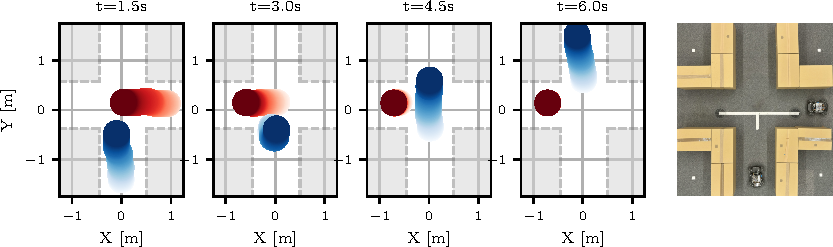
\includegraphics[width=0.9\linewidth]{figures/mar25_1_tracer_graph.pdf}

    \caption{Demonstration of multi-agent collision avoidance. Two robots are set 90° to each other in an intersection environment, with no direct view of the other robot and little visual overlap (right). The blue agent is given a goal pose on the other side of the intersection and successfully avoids a collision when the red agent is pushed through the intersection. The trajectories generated by the SLAM system are presented on the left charts.\captionbreak For visual reference, a video recording of the trials is available at 1m26s of the supplementary video\protect\footnotemark[1].}
    \label{fig:collision-avoidance}
\end{figure}
\footnotetext[1]{Supplementary video URL: \url{https://cam-diss.s3.amazonaws.com/video.mp4}}

\begin{figure}[h]
    \centering
    \captionsetup{format=plain, skip=0.5em}
    \begin{minipage}[b]{0.56\linewidth}
        \centering
        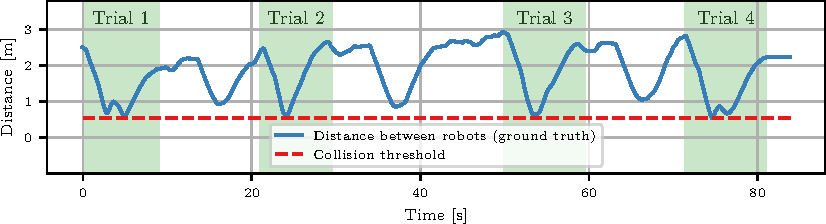
\includegraphics[height=1.6in]{figures/mar25_1_distance_plot.pdf}

        \caption{Plot of distance between the two robots throughout all four collision avoidance trials. The dips between trials are the robots' positions being reset.}
        \label{fig:collision-avoidance-distance-plot}
    \end{minipage}\hfill%
    ~
    \begin{minipage}[b]{0.42\linewidth}
        \centering
        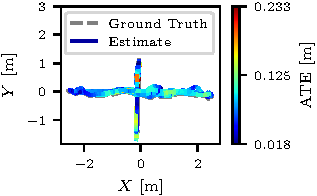
\includegraphics[height=1.6in]{figures/mar25_1_trajectory.pdf}
        \caption{Collision avoidance estimated trajectory and ground truth. The RMS abs.\ trajectory error is 0.074 meters.}
        \label{fig:collision-avoidance-traj}
    \end{minipage}
\end{figure}

% \subsection{Augmented Reality Visualization}
% \label{sec:augmented-reality-visualization-eval}
% My project included the development of an augmented reality visualization system to view my SLAM system's data overlayed on top of a video captured by an external camera. While no quantitative evaluation of this system will be performed, I believe it was a success as it performs its intended task of revealing how the map and trajectories generated by my system align with reality.

% More importantly, however, the tool is built around the standard ROS marker interface. This makes it a generic platform that can give an AR visualization of any experiment being conducted in a motion capture environment.

% A demonstration of the system can be found at 1m23s of of the supplementary video\footnote[1]{Supplementary video URL: \url{https://cam-diss.s3.amazonaws.com/video.mp4}}.